\documentclass[a4paper,10pt]{article}
\usepackage[utf8x]{inputenc}
\usepackage{amsmath}
\usepackage[margin=1.0in]{geometry}
\usepackage{algorithm}
\usepackage{algorithmic}
\usepackage{color}
\usepackage{epsfig}
\usepackage{multirow}
%\usepackage[pdftex,colorlinks=true,urlcolor=blue,pdfstartview=FitH]{hyperref}
\usepackage{tikz}
\usepackage{verbatim}
\usetikzlibrary{arrows,shapes}

\pdfcompresslevel=9
\usepackage{graphicx}
%\DeclareGraphicsExtensions{.png,.tif,.tiff}


\linespread{1.3}

%opening
\title{Ants for Dynamic Job Shop Scheduling Problem: Application to Harbor Logistics\thanks{Project Granted by the French DGE Agency (convention no 082930952)}}
\author{Ga\"{e}tan~Lesauvage\thanks{~Granted by French Ministry of Research}, Stefan~Balev, Fr\'{e}d\'{e}ric~Guinand\\\\
\medskip
Normandy University, LITIS EA 4108\\
BP 540, 76058 Le Havre, France\\
\medskip
E-mail: \{gaetan.lesauvage,stefan.balev,frederic.guinand\}@litislab.eu\\
\medskip
Phone: 0033 232 744 543
}


\begin{document}

\maketitle

%\newpage 

\begin{abstract}
%Container terminal and JSSP
In this paper we address the problem of Dynamic Job Shop Scheduling. This problem is stemmed from a real life application occuring in Harbor Logistics. On container terminals, special vehicles, called straddle carriers, continuously move containers, from trucks/train/ships to storage areas, from storage area to ships, trucks or train or directly from a ship to another one. Moving a container in the terminal is called a mission and is considered as a job. Such a job is composed of two operations: the pickup and the delivery. Each operation takes place in a particular and fixed location. Moreover, picking up and delivering containers have to be achieved within given time windows fixed according to external constraints. The overall objective is twofold: on the one hand we want to minimize the total distance covered by the straddle carriers, and on the other hand we want to minimize non respected time windows associated to each operation. 
%Dynamics
In addition, the terminal is subject to many dynamic events such as the arrival of unexpected missions, the update of some time windows, or vehicle failures for instance. For the dynamic version of the problem we have designed and implemented an ant-based approach for copping with such uncertainties, and we show that our algorithm performs quite well and provides near optimal solution in reasonnable computation time.
\end{abstract}

{\bf Keywords: } dynamic job shop scheduling problem, dynamic vehicle routing problem, ant colony optimization, ACO, container terminal, harbor logistics.\\

%=============================================================================
\section{Introduction}
%=============================================================================

%Contexte => Développement du transport conteneurisé
With the development of trade activities which have continually increased (from less than 6 millions of TEU in 1970 to 500 millions of TEU in 2008\footnote{Source: Containerization International (http://www.ci-online.co.uk)}), container has become the first mode of packaging for exchanging goods. One of the cheapest way to carry thousands of tons of goods around the world are containers vessels which are able to carry at once ten of thousands containers. As a consequence, multimodal platforms have been created all around the world in order to facilitate the transfer between ships and trucks or trains. In order to reduce the costs of these transferts, the harbor has to provide a high quality of service and unceasingly develop new technologies and processes. The present work focuses on one particular point of the organization of container terminals: the scheduling of straddle carriers missions.\\

Schematically a container terminal is divided into 5 areas : the yard composed of lanes of stacked containers, the depot where the idle vehicles are parked, the trucks area, the trains area and the quays.

%Environnement => Terminal à conteneur : définitions des termes relatifs au conteneurs et à leur transport
Straddle carriers are used within the terminal to move containers. Those vehicles can lift a container from above and designed for moving containers in the yard by driving over the lanes. They are also used to load or unload trucks or trains. Some of them are able to dynamically adapt the spreader\footnote{grip use to grab container} size to any container dimensions while some of them require to be set up in the depot.\\%Cout unitaire extremement eleve + Conso fuel enorme => 


Moving a container requires a straddle carrier to pickup, to move from one place to another one and to deliver the container once arrived at destination. This set of handling and moving is called a mission. There are four kinds of missions:
\begin{itemize}
	\item Incoming container missions;
	\item Outgoing container missions;
	\item Transshipment missions;
	\item Yard container missions.
\end{itemize}

\begin{figure}[ht]
  \begin{center}
  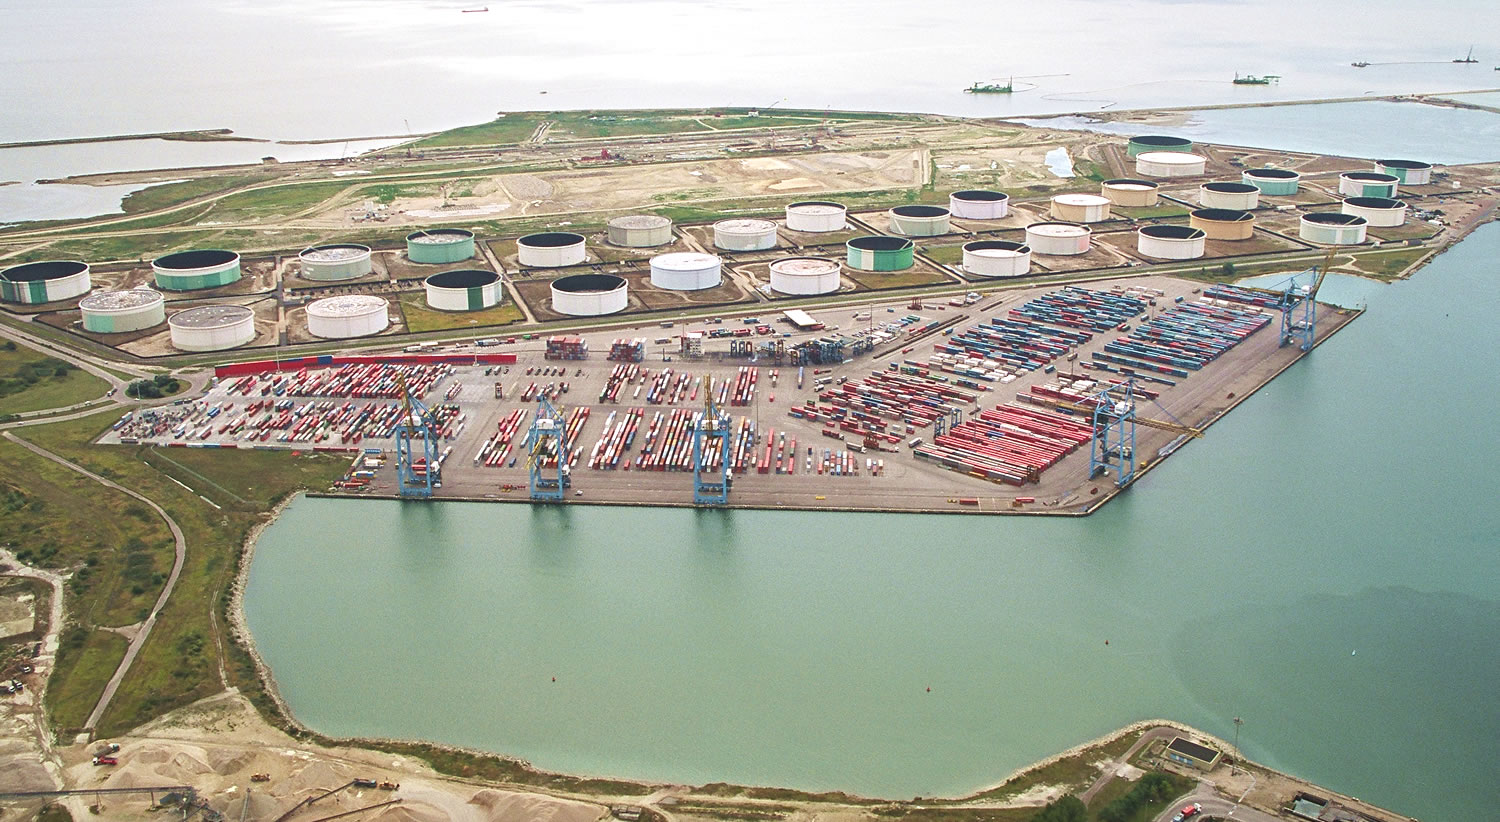
\includegraphics[width=0.6\textwidth]{Figures/terminalOfNormandy}
  \caption{The Terminal of Normandy, Le Havre's harbor, France.}
\end{center}
\end{figure}


The first mission type concerns trucks, trains and ships unloading. Straddle carriers drive to the pick-up locations to unload the vehicles, and then lift the container, drive to the yard to stock it. Concerning ships, they are unloaded by quay cranes which stack containers on the quay. Then, straddle carriers come to pick-up the containers and move them to the yard.
The second category concerns trucks, trains and ships loading. In this case, straddle carriers start by picking-up a container from the yard and then drive to the delivery location (trucks areas, trains area or ship areas) to deliver it to their recipient. 
The third category of missions concerns the move of a container from a ship to another one.
Finally, the last kind of missions concerns internal yard optimization process. Indeed, in some cases, it can be useful to reorganize part of the storage area in order to reduce further delivery times or to free strategic container slots for next unloading missions.\\

Each mission is composed of a pickup phase, a moving phase and a delivery phase. The first and last phases are each constrained by a time window. These time windows correspond to appointments between straddle carriers and customer vehicles (trucks, trains or ships). Straddle carriers have to reach the pickup or delivery location within the given time window. If a straddle carrier comes too early, it will have to wait. On the contrary, if it comes too late, the customer vehicle will have to wait and may require late fees from the container terminal exploitation compagny. Thus, overrunning a time window implies a cost for the container terminal. Note that, in the case of yard optimization missions, time windows can be overrun without entailing penalties or additional costs. So, according to the mission kind, time windows can be hard or soft. For incoming missions, the pickup time window is hard and the delivery time window is soft. For the outgoing container missions, the pickup time window is soft but the delivery time window is hard. For transshipment missions, both time windows are hard, and for yard optimization missions both time windows are soft. 

%Définition du problème => Affectation et ordonnancement de missions aux chariots cavaliers.
On the terminal, straddle carriers perform missions one after the other with a double objective: respecting missions time windows and minimizing the overall covered distance \cite{Lesauvage2009}. Indeed, time windows must be respected to avoid penalty fees and the distance covered by the vehicles directly impacts the exploitation costs of those vehicles. %//CONSO FUEL ?
So, part of the problem may be expressed as a static scheduling problem.
%in terms of So, the optimization problem discussed in this paper concerns the allocation and the scheduling of the missions to the straddle carriers.\\
%Aspect dynamique et incertitude
However, in real life, container terminals are subject to dynamic events occuring in an unpredictible way. New missions are added to the system for answering custoners needs. Some customers may also miss the time windows, some straddle carriers may suddenly become unavailable or some lanes may be closed temporarily.
Such dynamic uncertainties contribute to the unpredictible evolution of the environment.

As a consequence, the feasibility of a fully static schedule is unlikely. The work presented in this parper focuses on the allocation and the scheduling of the missions to the straddle carriers. The ant based method proposed aims at providing feasible solutions that are continously reoptimized in response to dynamic events.

%Plan
The next section presents the modeling of the problem for both static and dynamic formulations and exposes related existing works. Section \ref{sec:ants} is devoted to the main contribution of this paper, a swarm intelligence method, based on the ant metaphor able to cope with dynamic events, for generating relevant schedules. Section \ref{sec:expe} presents and discusses results obtained by the method on both static and dynamic versions of the problem. A final section concludes this work and opens some perspectives.

%In this paper we will first describe the modeling the straddle carriers scheduling problem in its static and dynamic form. Then we will propose an ant colony based algorithm to solve it. Finally, we will discuss about the performance of this approach.

%=============================================================================
\section{Problem Modeling and Related Works}
%=============================================================================

%We will give here the modeling of the problem in its static and dynamic version.

In the static as well as in the dynamic version, the problem is considered for a fixed and limited period of time that will be called "day", for simplicity, in the sequel. It has to be noticed that on most containers terminals the activity is an ever-going process (24 hours a day, 7 days a week) justifying and motivating the design and implementation of optimization processes able to cope with dynamic events. 

%=========================================================================
\subsection{Problem Modeling}
%=========================================================================

%Characteristics
In its static version, we assume that no dynamic event can occur during the day. The number of straddle carriers is supposed to be known and fixed for the whole day. This implies that, once computed a schedule remains valid. As additional hypothesis we suppose that the travel time between two locations within the container terminal is known and does not vary during the day. Moreover, we also assume that time windows are respected by the customers for both pickup and delivery. Finally all missions that are planned during the day are supposed to be known a priori. \\

%--------------------------------------------------------
%\subsubsection{General Formulation}
%--------------------------------------------------------

%In our context, scheduling missions for straddle carriers, the 
According to the introduction, the problem may be formulated as a job shop scheduling problem (JSSP) in which the machines are the straddle carriers and the missions are the jobs. \\

The problem consists in finding the schedule $S$ of $n$ jobs $J_i$~$(i=1,\ldots,n)$ on $m$ machines $M_j$~$(j=1,\ldots,m)$. This schedule is represented by the workload $W_{M_j}$ of each machine $M_j$. The workload $W_{M_j}$ is an ordered list of jobs allocated to the machine $M_j$. Each job is made of two operations: $O_1$: pickup of the container and $O_2$: delivery of the container. As $O_1$ and $O_2$ operate on the same container, they have to be processed on the same machine (the straddle carrier) in this order. Moreover, between the execution of both operations, the vehicle has to move from one place (the pickup location) to another place (the delivery location) and this movement entails a delay between $O_1$ and $O_2$ related to the distance between both locations.

% SCHEDULE EQUATION
\begin{equation*}
\begin{cases}
 S = \{ W_{1} , W_{2} \ldots , W_{m}\} & \text{and}\\
 W_{i} = \{ J_{\alpha_1} , \ldots , J_{\alpha_k} \} & \text{with $k \leq n$, and $W_{i} \cap W_{j} = \emptyset$,  $\forall i \neq j$} 
\end{cases}
\end{equation*}
 
%Setup Costs
%----------------------------------------------------
%\subsubsection{Setup times and distances}
%----------------------------------------------------

For starting a mission, the straddle carrier has to move to the pickup location. This move can be considered as a setup time or cost. This setup time directly depends on the location of the straddle carrier at the end of the previous mission, if any. If a previous mission was executed by the straddle carrier, then the distance used for computing the setup time is equal to the distance between the delivery location of the previous mission and the pickup location of the current one. If no mission was executed before, then the straddle carrier is supposed to be located at the depot. As a consequence, setup times are sequence dependent ($ST_{sd}$). 

Let us consider two jobs, $J_i$ and $J_j$ each composed of two operations, $O^i_1, O^i_2$ and $O^j_1, O^j_2$. Each operation has to be performed on a precise location on the terminal. Let us denote by $l(O^k_p)$ the location of the operation $p$ ($p \in \{1,2\}$) of job $J_k$. Then, if a machine is allocated both jobs in the order ($J_i, J_j$), then the setup cost $setup_{i,j}$ is proportional to $d(l(O^i_2),l(O^j_1))$ where $d(l,l')$ denotes the shortest path between the locations $l$ and $l'$. As the machines are supposed to move at the same speed, we consider that the travel time (setup cost) for chaining job $J_i$ to job $J_j$ on the same machine is equal to $t(d(l(O^i_2),l(O^j_1)))$. Note that, if the machine performs job $J_i$ coming from the depot, the setup is proportional to: $d(\mbox{depot},l(O^i_1))$.

%---------------------------------------------------------
\subsubsection{Other Assumptions}
%---------------------------------------------------------

% Pas de préemption
In all generality, the machines may be heterogeneous, depending on their spreader size and adaptability, such that a job $J_j$ may not be compatible with machine $M_i$. For instance, if the straddle carrier has a spreader only adapted to 40 feet containers, then it will not be able to process 20 feet containers missions. However, such cases have not be considered in the current work. In addition in the static form of the problem and for sake of simplicity, we consider that the speed of all the machines is equal. \\

%\subsubsection{Preemption}
%There is no preemption here since the delivery can not be done without picking up the container before.
No preemption is allowed in the straddle carrier mission scheduling problem. Preemption of a mission can only be considered during the movement phase. Indeed, both pickup and delivery are atomic operations. Thus, preempting a mission is equivalent to stopping the vehicle along the way from the pickup location to the delivery location. And stopping the mission entails an "intermediate delivery" of the container on a temporary location, followed later by picking up again the same container from that location to the final delivery one. Thus, preempting a mission can be considered as the transformation of one mission into two new missions. While such a situation is sometimes observed in real life, we assume that no mission can be split into several ones in the context of the present work.\\

%\subsubsection{Precedence}
% //Pas de Precedence
The jobs are independent in the problem, there is no precedence constraint between them. Though, operations are constrained by time windows. So, if two jobs are scheduled successively without taking into account their time windows, those time windows can be exceeded. In the case of two missions concerning the same delivery slot in the container terminal, if the container of the second mission must be stacked onto the container of the first mission, then the first job should be achieved before the second one. But if the second job is processed before the first one, then a new mission will be added in the pool of jobs to switch the two containers. Again, in the context of the present work, such situations are ignored. %So, in this particular case, the time windows of these missions should take into account the precedence between the jobs.\\


\begin{figure}[h]
\label{example}
 \tiny
 \begin{center}
    \begin{tabular}{|c|c|c|c|c|} 
    \hline
    {\bf Missions} & \multicolumn{2}{|c|}{\bf Pickup TW} & \multicolumn{2}{|c|}{\bf Delivery TW} \\ \hline
    $M_1$	 & $00:01:09$ & $00:03:17$	& $00:03:52$ & $00:06:00$\\
    $M_2$	 & $00:01:32$ & $00:04:10$	& $00:04:35$ & $00:06:47$\\
    $M_3$	 & $00:07:10$ & $00:09:52$	& $00:09:14$ & $00:12:20$\\
    \hline

    \end{tabular}
\end{center}
\begin{center}
    \begin{tabular}{|c|c|} 
    \hline
    {\bf Vehicle} & {\bf AVG Speed (km/h)} \\ \hline
    $V_1$	 & $20$\\
    $V_2$	 & $25$\\
    
    \hline

    \end{tabular}
  \end{center}
  
  \begin{center}
    \begin{tabular}{|c|c|c|c|c|} 
    \hline
    \multirow{2}{*}{\bf{Origin}} & \multicolumn{4}{c|}{\bf{Destination}}\\ \cline{2-5}
    	 	& {\bf $Depot$}	& {\bf $M_1$}	& $M_2$		& $M_3$\\ \hline
    {\bf $Depot$}	& $0$		& $173$		& $334$		& $328$\\
    {\bf $M_1$}		& $347$		& $306$		& $642$		& $636$\\
    {\bf $M_2$}		& $344$		& $317$		& $413$		& $407$\\
    {\bf $M_3$}		& $348$		& $399$		& $399$		& $396$\\
    \hline
    \end{tabular}

  \end{center}

  \begin{center}
    \begin{tabular}{|c|c|c|c|c|c|c|c|c|} 
    \hline
     \multirow{3}{*}{\bf{Origin}}	& \multicolumn{8}{c|}{\bf{Destination}}\\ \cline{2-9}
	& \multicolumn{2}{c|}{$Depot$}	& \multicolumn{2}{c|}{$M_1$}	& \multicolumn{2}{c|}{$M_2$}		& \multicolumn{2}{c|}{$M_3$}\\ \cline{2-9}
    	 	& $V_1$ & $V_2$	& $V_1$ & $V_2$ & $V_1$ & $V_2$ & $V_1$ & $V_2$\\ \hline
    {\bf $Depot$}	& $00:00:00$	& $00:00:00$		& $00:00:31$ & $00:00:25$		& $00:01:00$ & $00:00:48$		& $00:00:59$	& $00:00:47$\\
    {\bf $M_1$}		& $00:01:02$	& $00:00:50$		& $00:00:55$ & $00:00:44$		& $00:01:56$ & $00:01:32$		& $00:01:54$	& $00:01:32$\\
    {\bf $M_2$}		& $00:01:02$	& $00:00:50$		& $00:00:57$ & $00:00:46$		& $00:01:14$ & $00:00:59$		& $00:01:13$	& $00:00:59$\\
    {\bf $M_3$}		& $00:01:03$	& $00:00:50$		& $00:01:12$ & $00:00:57$		& $00:01:12$ & $00:00:57$		& $00:01:11$	& $00:00:57$\\
    \hline
    \end{tabular}
  \end{center}
\begin{center}
  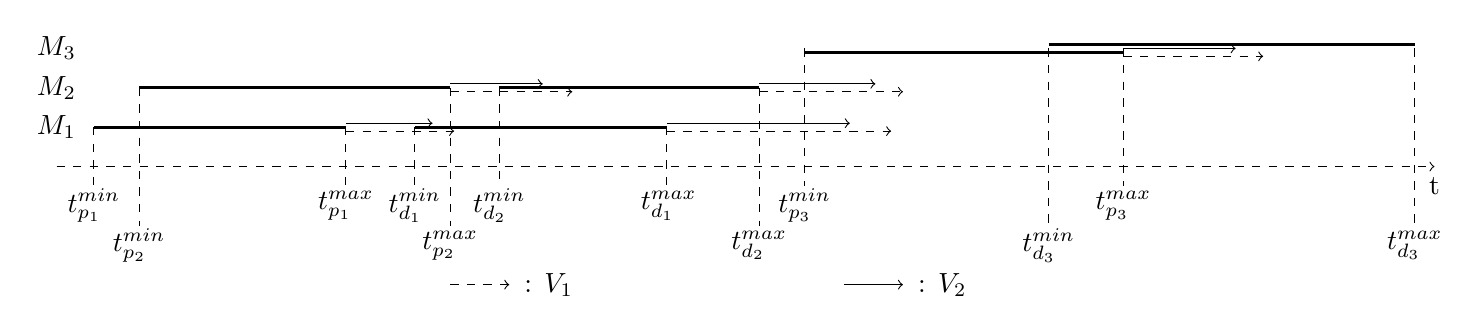
\begin{tikzpicture}[-,thick,xscale=0.25,yscale=0.5]
    \tikzstyle{v1}=[thin,dashed,->]
    \tikzstyle{v2}=[thin,->]
    \tikzstyle{tw}=[very thick,-,black]
    \tikzstyle{time}=[thin,dashed,->]
    \tikzstyle{trait}=[thin,dashed]

    \node (M1) at (5,1) {$M_1$};
    \node (M2) at (5,2) {$M_2$};
    \node (M3) at (5,3) {$M_3$};
    
    %M1
    \draw[tw] (6.9,1) -- (19.7,1);
    \draw[tw] (23.2,1) -- (36.0,1);
    %M2
    \draw[tw] (9.2,2) -- (25,2);
    \draw[tw] (27.5,2) -- (40.7,2);
    %M3
    \draw[tw] (43,2.9) -- (59.2,2.9);
    \draw[tw] (55.4,3.1) -- (74.0,3.1);

    %M1 : P -> D
    \draw[v1] (19.7,0.9) -- (25.2,0.9);
    \draw[v2] (19.7,1.1) -- (24.1,1.1);
    %M1 -> M3
    \draw[v1] (36,0.9) -- (47.4,0.9);
    \draw[v2] (36,1.1) -- (45.3,1.1);
    %M2 : P -> D
    \draw[v1] (25,1.9) -- (31.2,1.9);
    \draw[v2] (25,2.1) -- (29.7,2.1);
    %M2 -> M3
    \draw[v1] (40.7,1.9) -- (48,1.9);
    \draw[v2] (40.7,2.1) -- (46.6,2.1);
    %M3 : P -> D
    \draw[v1] (59.2,2.8) -- (66.3,2.8);
    \draw[v2] (59.2,3.0) -- (64.9,3);
    
    \draw[time] (5,0) -- (75.0,0);

    \draw[trait] (6.9,1) -- (6.9,-0.5);
    \draw[trait] (19.7,1) -- (19.7,-0.5);
    \draw[trait] (23.2,1) -- (23.2,-0.5);
    \draw[trait] (36,1) -- (36,-0.5);
    
    \draw[trait] (9.2,2) -- (9.2,-1.5);
    \draw[trait] (25,2) -- (25,-1.5);
    \draw[trait] (27.5,2) -- (27.5,-0.5);
    \draw[trait] (40.7,2) -- (40.7,-1.5);

    \draw[trait] (43,3) -- (43,-0.5);
    \draw[trait] (59.2,3) -- (59.2,-0.5);
    \draw[trait] (55.4,3) -- (55.4,-1.5);
    \draw[trait] (74,3) -- (74,-1.5);

    \node (m1PMin) at (6.9,-1) {$t_{p_1}^{min}$};
    \node (m1PMax) at (19.7,-1) {$t_{p_1}^{max}$};
    \node (m1DMin) at (23.2,-1) {$t_{d_1}^{min}$};
    \node (m1DMax) at (36.1,-1) {$t_{d_1}^{max}$};
    
    \node (m2PMin) at (9.2,-2) {$t_{p_2}^{min}$};
    \node (m2PMax) at (25,-2) {$t_{p_2}^{max}$};
    \node (m2DMin) at (27.5,-1) {$t_{d_2}^{min}$};
    \node (m2DMax) at (40.7,-2) {$t_{d_2}^{max}$};

    \node (m3PMin) at (43,-1) {$t_{p_3}^{min}$};
    \node (m3PMax) at (59.2,-1) {$t_{p_3}^{max}$};
    \node (m3DMin) at (55.4,-2) {$t_{d_3}^{min}$};
    \node (m3DMax) at (74,-2) {$t_{d_3}^{max}$};

    \node (t) at (75,-0.5) {t};

    \draw[v1] (25,-3) -- (28, -3);
    \draw[v2] (45,-3) -- (48,-3);

    \node (v1Legend) at (30, -3) { : $ V_1$ };
    \node (v2Legend) at (50, -3) { : $ V_2$ };
  \end{tikzpicture}

\caption{Example of a problem with 2 machines ($V_1$ and $V_2$) and 3 jobs ($M_1$, $M_2$ and $M_3$).}
\end{center}
\end{figure}


%---------------------------------------------------------
\subsubsection{Optimization criteria}
%---------------------------------------------------------

Two main criteria are taken into account for optimizing the scheduling of straddle carriers missions on container terminals: the distance traveled by all the straddle carriers, and the respect of the constraints induced by jobs pickup and delivery time windows.\\

The distance covered by the machines depends on both the distance between the pickup and the delivery places and also the distance between the location of the end of a job to the location of the beginning of the next one. Thus, for each sequence of jobs ($J_i,J_j$) performed by a machine, the covered distance is equal to $d(l(O^i_2), l(O^i_1))$ plus the distance $d(l(O^j_1), l(O^j_2))$. If $J_i$ is the first job executed by the machine, then the distance is equal to $d(l(\mbox{depot}),l(O^i_1))$ and if the job $J_j$ is the last job executed then an additional distance should be added to the total distance covered by the machine: $d(l(O^j_2),l(\mbox{depot}))$.

%\subsubsection{Tardiness}
%Tardiness
The second criterion is related to time windows associated to job operations. If a mission misses one or both of its time windows, then there is tardiness. Total tardiness for a job $J_i$ allocated to machine $M_k$ is the sum of pickup tardiness $T^k_{i,O_1}$ and delivery tardiness $T^k_{i,O_2}$. The pickup tardiness is the difference between the arrival time of $M_k$ at the pickup location of $J_i$ and the end of the pickup time window of $J_i$. The delivery tardiness is the difference between the arrival time of $M_k$ at the delivery location of $J_i$ and the end of the delivery time window of $J_i$. \\

Let us consider that machine $M_k$ executes the sequence ($J_i,J_j$), and that the delivery operation of job $J_i$, performed by $M_k$, ends at $C^k_i$. We also denote the time needed to travel from location $l$ to $l'$, $t(d(l,l'))$ (as for the setup times). We also denote by $tw_{min}(O^i_1)$ (resp. $tw_{max}(O^j_2)$) the starting date (resp. ending date) of the time window of the pickup (resp. delivery) operation of job $J_i$ (resp. $J_j$). Then, the tardiness for job $J_j$, executed by $M_k$, may be expressed as follows: 
%TARDINESS FORMULA
\begin{equation*}
 \begin{cases}
    T^k_{j,O_1} = max(0, (C^k_i + t(d(l(O^i_2),l(O^j_1)))) - tw_{max}(O^j_1)) = max(0,C^k_i+setup_{i,j}-tw_{max}(O^j_1))\\
    T^k_{j,O_2} = max(0 ,C^k_j - tw_{max}(O^j_2))\\
    T^k_{j} = T^k_{j,O_1} + T^k_{j,O_2}
\end{cases}
\end{equation*}

The tardiness may entail some penalty costs to the container terminal. Depending on the kind of mission, these costs may be more or less important. This can be represented by weighted tardiness. For summarizing, the optimization aims at minimizing two criteria, the total distance covered by the vehicles and the total weighted tardiness. 

If we consider $n$ jobs, and if we denote $M(i)$ the machine performing job $J_i$, the tardiness function to minimize can be expressed as follows:

%According to the kind of mission, the tardiness may cause penalty costs to the container terminal customers. These potential penalties can be seen like weighted tardiness and the best schedule is the one minimizing this weighted tardiness.
%WEIGHTED TARDINESS FORMULA
\begin{equation*}
    F_S = \sum_{j=1}^{n}(w_j.T^{M(j)}_{j})
\end{equation*}
 
%Always in order to reduce exploitation costs and once the weighted tardiness has been minimized, the goal is to minimize the distance covered by the vehicles. So, the second criteria to minimize is the process cost of the tasks.
The total distance covered by the machine $M_i$ is equal to: 
%and if we assume that $m$ represents the number of machines, the workload on machine $M_i$ is represented by  $W_{i} = \{ J^i_1 , \ldots , J^i_k \}$, with $k \leq n$, and $W_{i} \cap W_{j} = \emptyset$,  $\forall i \neq j$, and the schedule is: $S = \{ W_{1} , W_{2} \ldots , W_{m}\}$. Then, the total distance covered by a machine $M_i$ is equal to: 

\begin{equation*}
    D_i = d(l(\mbox{depot}),l(O^1_1)) + d(l(O^1_1),l(O^1_2) + \sum_{k=2}^{card(W_i)} \left( d(l(O^{k-1}_2),l(O^k_1)) + d(l(O^k_1),l(O^k_2)) \right) + d(l(O^{card(W_i)}_2),l(\mbox{depot}))
\end{equation*}

where $card(W_i)$ denotes the number of jobs in the workload of the machine $i$. 

The total distance covered by all the machines can be expressed as: 

%PROCESS COST FORMULA
\begin{equation*}
    D_S = \left(\sum_{i=1}^{m} D_i\right)
\end{equation*}

Since the allocation of the jobs to the machines influence the distance covered by the vehicles, the criteria $F_S$ and $D_S$ are not independent. The algorithm we propose in the next section uses a weighted combination of those criteria.

%=====================================================================
\subsubsection{Related works}
%=====================================================================	

It should be noticed first that if we relax the time windows constraints, the problem may be formulated in the following terms: given a set of tasks, such that each task is composed of a pickup operation, a movement between two places (a source and a destination) and a delivery operation, how to allocate the tasks to vehicles such as to minimize the covered distance? \\%This problem is evidently related to the class of vehicle routing problem (VRP). 


	%	VRP -> VRP-TW -> PDP-TW
Since the problem is about finding shortest routes for a fleet of vehicles, it seems natural to look at existing works dealing with Vehicle Routing Problems (VRP) \cite{Toth2001,Laporte1992} and more precisely dealing with Pickup and Delivery Problem (PDP) \cite{Berbeglia2007}. This latter version of VRP consists in picking up goods before delivering them to the customers. A variant of PDP takes into account the time windows \cite{Mitrovic1998}. Here, the pickup and the deliveries must occur into given time intervals. There is also a version of these problems with vehicles characterized limited capacities \cite{Toth2001}. \\

%DIRE pq c pas un VRP, PDP, ou m-TSP TW
In those problems each vehicle usually has a fixed capacity greater than one and the problem is to find shortest paths to deliver the goods to the customers. In our problem, each vehicle has a unit capacity. This means that only one delivery per pickup operation is possible. Moreover, in our problem a given customer requires only one type of good, located at a given fixed place, such that no choice is possible for the pickup location and the delivery one. Our main issue is related to the way the missions are chained one after the other on each vehicle, and a solution of this problem is highly constrained by the pickup and delivery time windows. Thus, our problem seems to be more related to job shop scheduling than to vehicle routing.\\

	%	JSSP -> JSSP with ST_SD and R_SD
  %STATE OF THE ART OF USED METHODS IN JSP, JSP-ST_{sd}, DJSP													   %JSP-ST_{sd}
For the Job Shop Scheduling Problem (JSSP) a set of $n$ jobs is given as well as a set of $m$ machines. Each Job $J_i$ consists of a sequence of $k_i$ operations that have to be performed in this order on different machines. Each operation is characterized by a processing time that may depend on the machine it is allocated to. In addition, a machine can process only one operation at a time and a given operation can only be processed by a single machine at a time. \\


The literature about the JSSP is huge and we invite the reader to refer to the work of Jain et al. \cite{Jain1999} for a general and comprehensive survey about this problem. The short state of the art presented in the sequel focuses specifically on ant based methods dealing with JSSP since such an approach has been chosen for addressing the current problem.\\

In \cite{Jain1999} and \cite{Brucker2010}, the authors give a survey of Job Shop Scheduling Problems and of the methods used to solve the different sub-problems.
%JSP and ACS
Among the different methods used for solving the problem, an ant system algorithm has first been introduced by Colorni et al. \cite{Colorni1994}. The authors used a complete graph representing the possible schedules and tabu lists to mark the nodes (jobs) chosen by the ants. When all the jobs are in the tabu list, the solution represented by the list is evaluated by a fitness function. The authors concluded that Ant Colony algorithms are one of the most easily adaptable population based algorithm. More recently, Apinanthana et al. extended the use of Ant Colony based algorithm to solve the Multi-criteria Job Shop Scheduling Problem \cite{Apinanthana2011}.
%JSP-TW
In \cite{Huang2008}, the authors proposed a corresponding algorithm for the Job Shop Scheduling Problem with Time Windows (JSSP-TW). They showed that Ant Colony Optimization is both efficient and effective for this class of optimization problems.

%FJSP
In the Flexible Job Shop Scheduling Problem (FJSSP), all the machines are able to process any operation. This version of the Job Shop Scheduling problem has been first introduced by Brucker and Schlie in \cite{Brucker1990}. They proposed a graphical methods for solving this problem with two jobs. Since the problem is NP-Hard for more than two jobs, meta-heuristics have been used. In \cite{Ponnambalam2005}, Ponnambalam et al. introduced an Ant Colony Optimization algorithm to solve large instances of the FJSSP up to 20 jobs and 15 machines. In \cite{Xing2010}, Xing et al. used a hybrid optimization method to solve the FJSSP using both knowledge and Ant Colony Optimization models. The algorithm memorizes good features of past iterations to guide the ACO algorithm toward best solutions.

In \cite{Allahverdi2008} the authors give a survey of algorithms used to solve Job Shop Scheduling Problems with Sequence Dependent Setup Times (JSSP-SDST). Many different methods have been used for that problem: hybrid genetic algorithms, disjunctive graphs, mixed integer linear programming model with local search scheme, fast tabu search, branch and bound, dynamic programming, polynomial insertion algorithm, Lagrangian relaxation or ant colony algorithms. In \cite{Taillard1994}, Taillard developped a tabu search algorithm for the JSSP. This algorithm has been improved along the time (\cite{Blazewicz1996, Watson2003}) and is known to be one of the most effective technique to solve the JSSP. Simulated Annealing (SA) or Genetic Algorithms (GA) are also widely spread to generate solutions to the JSSP.\\% and without removal time sequence dependent criteria.\\

However most of these methods can only been applied to a static version of the JSSP-SDST problem.

%=========================================================================
\subsection{Dynamic version of the problem}\label{subsec:dynamic}
%=========================================================================

	%Characteristics
In its dynamic version, the straddle carriers scheduling problem takes into account dynamic events. It implies that a computed schedule can become deprecated during the day. Many different dynamic events may occur during the execution of the schedule. According to \cite{Ouelhadj2009}, dynamic events are either resource or job related. For instance, the travel times between each location within the container terminal, which are known a priori, may vary during the day. The number of straddle carriers, known at the beginning of the day, can change since some of them can become unavailable for whatever reason. Time windows can also be subject to some modifications if, for instance, a truck, or a ship, is in late for meteorological reasons. And last, but not least, some new missions may arrive at any moment of the day, without prior notice.\\

	%	DVRP -> DVRP-TW -> DPDP-TW
Some of these situations have already been studied. For instance, Berbeglia et al. described the dynamic version of pickup and delivery problems in \cite{Berbeglia2010}. However, in their work they do not consider time windows. This temporal constraint is present in the work of S. Mitrovic-Minic \cite{Mitrovic2001}. She addressed the problem of Dynamic Pickup and Delivery with Time Windows (DPDP-TW). In \cite{Mitrovic2006}, S. Mitrovic-Minic and her colleagues used a multiple Traveler Salesman Problem (m-TSP) formulation of the Vehicle Routing Problem with Time Windows (VRP-TW). They used precedence graphs to model the multiple Traveler Salesman Problem with Time Windows (m-TSPTW). They proposed algorithms to compute bounds on the number of vehicles required to complete the deliveries. They also showed that this problem is NP-Hard.\\

The problem of Job Shop Scheduling, when new jobs must be inserted into a pre-computed schedule, is known as the Dynamic Job Shop Scheduling Problem (DJSSP) \cite{Ramasesh1990}.

%State of the art?
In \cite{Ouelhadj2009}, the authors distinguish four different approaches to the dynamic version of the problem: completely reactive scheduling, predictive reactive scheduling, robust predictive-reactive scheduling, or robust pro-active scheduling. Suresh and Chaudhuri, in \cite{Suresh1993}, regroup theses approaches in two classes: predictive and reactive scheduling. In reactive scheduling, the schedule is computed according to the events. The most common strategy is the predictive and reactive scheduling where a schedule is first computed, and then updated according to the events. On the other hand, in predictive scheduling, the schedule is computed in the way that it facilitates the handling of possible dynamic events.

%When reschedule
Each of these strategies requires rescheduling. According to Oulhadj and Petrovic in \cite{Ouelhadj2009}, three different policies can be found in the literature: the periodic rescheduling, the event driven rescheduling, and a hybrid rescheduling which is a combination of the two other policies. The authors explain that the periodic policy can be sufficient to deal with the dynamic events, but that the size of the period should be determined carefully. Besides, the authors concluded that in every studyied paper of their survey, the event driven policy gives better results than the periodic policy.

%Which stratedy
Since the objective of the reschedule is to take into account the new characteristics of the problem, two strategies can be used: either reschedule from scratch or repair the previous computed schedule \cite{Ouelhadj2009}. The first strategy appears to be unusable in practice because of the lack of time to compute the whole new schedule.

%Which way ?
As for dynamic vehicle routing problems, exact algorithms can not be used anymore to compute the schedule, due to the lack of time between jobs arrivals. Several studies have been carried on heuristics and meta-heuristics methods, AI based techniques and multi-agent approaches to solve the DJSSP.
%Heuristics
In \cite{Gere1966}, Gere introduced heuristics for both JSSP and DJSSP. He tested the efficiency of each heuristic and showed that the choice of the good heuristic is more important for solving the problem than the choice of a priority rule for the jobs. He concluded that heuritics based on anticipation of the schedule improved significantly the quality of the solution while only slightly raising the computing time.
%AI
Artificial Intelligence based methods are also used for DJSSP, such as knowledge based algorithms, neural networks, case based reasoning, fuzzy logic or petri nets.
%SMA
More recent approach using Multi-Agent Systems (MAS) to provide solutions has been developed. In \cite{Yoo2002}, Yoo and M\"{u}ller introduced a MAS using a simulated annealing algorithm to optimize the solutions proposed by the agents.
%Meta Heuristics
Regarding meta-heuristics, they represent the most common way to provide solutions for DJSSP. Genetic Algorithms are one of the most used meta-heuristics to solve the dynamic version of the problem (\cite{Lin1997, Qi2000}).
%ACO
Despites the use of Ant Colony algorithms for solving the static versions of Vehicle Routing and Job Shop Scheduling problems, only a few researches have been applied to the dynamic versions of these problems. Vogel et al. proposed a continously operating Ant algorithm to solve the Real World Shop Floor Scheduling Problem \cite{Vogel2002}. They concluded that their algorithm does not achieve the quality of the Genetical Algorithm solution but that it will lead further research on Ant algorithms toward better results.
In \cite{Montemanni2005}, Montemanni et al. introduced an Ant Colony System (ACS) for solving the Dynamic Vehicle Routing Problem. They applied their algorithm to a realistic test case study of fuel distribution in the city of Lugano in Switzerland. They showed that their ACS provides good solutions on both theorical and real problems.
More recently, Zhou et al. applied an Ant Colony Optimization algorithm to the Dynamic Job Shop Scheduling Problem \cite{Zhou2008}. They perform their algorithm on two problems having the same jobs to complete but different degree of dynamism. They showed that the algorithm gives good results in both cases.\\



%As showed above, the proposed schedule must be failsafe and has to deal with variations of the environment. \\
	%	DJSSP -> DJSSP with ST_SD and R_SD
	%	On-line algorithm
																				      %Motivation 
We propose in the next section an on-line ant colony based algorithm able to propose near optimal solutions at any time for the problem in its dynamic version. The present work is motivated by the lack of studies about the DJSSP with time windows and sequence dependent setup time. Moreover, we aim at minimizing the total distance covered by the machines and the tardiness where  most of the algorithms in the literature focus on minimizing the makespan.

%=============================================================================
\section{Colored Ants algorithm}\label{sec:ants}
%=============================================================================

Bio-inspired algorithms have been more and more used for providing solutions for hard optimization problems since the early nineties \cite{Dorigo2006}. Ant-based approaches (Ant System, Ant Colony Optimisation, Ant Colony System), take advantage of some properties and characteristics that have been discovered by entomologists and sometimes have been reproduced through experiments, as it was done by Deneubourg in 1983 \cite{Deneubourg1983}, that showed stigmergy between ants. Ant-based or stigmergic systems are particulary well adapted to dynamic optimization problems because of some of their intrinsic characteristics like: decentralized control, indirect communications (entailing positive feedback), and the possibility of forgetting outdated solutions thanks to a bio-inspired mechanism: the evaporation of the pheromone tracks (entailing a negative feedback).\\

Our method relies on multiple colonies of ants. In our version, ants are attracted by pheromones of their own colony and repulsed by pheromones of foreign colonies. This mechanism results in a collaboration between the ants of a colony and a competition between the different colonies. The idea consists in making them compete for having access to jobs that are compatible, in terms of time windows.\\

A similar approach has been designed and implemented by Bertelle et al. in \cite{Bertelle2006,Bertelle2007} for determining dynamically the best distribution of a parallel program on a network. They used a collaboration/competition process between colonies of artificial ants to distribute the data and the computations of a program among heterogeneous processing ressources while minimizing the communication overhead between computing ressources. The authors used a threshold to avoid ants from choosing a destination containing too much ants entailing an implicit mechanism of repartition of the ants over the search space. Instead of using a threshold that might be difficult to tune correctly, we will see below that we choose a linear combination of the repulsion aspect in the pseudo-random-proportional transition rule.\\

In our model, a colony represents a vehicle (machine). The vehicle has to choose the best sequence of missions to process, the one that both minimizes weighted tardiness and the covered distance. We modeled the \textcolor{red}{different solutions}\footnote{que veux-tu dire ?} as paths on a graph. The ants of the colony have to colonize the mission graph in order to find the shortest path from the source node to the sink. When an ant moves to a node (corresponding to a mission), it drops pheromone according to the quality of the marked node. This pheromone will be used to guide other ants of the colony toward the node and to repulse ants of other colonies to other nodes. As each colony has the same behavior, the nodes are partitioned between the different colonies and this distribution tends to minimize the overall covered distance of the vehicles.\\

Each colony is modeled by a color. In this way, each node of the graph is colored by the color of the highest amount of pheromone on this node. The solution is obtained by constructing the best paths for each color. Each path $P_i$ of color $i$ is built by starting at the source node and by searching among the set $S_{j,i}$ of accessible nodes colored in $i$ the node with the highest level of pheromone. The process is repeated until either the sink node has been reached or the $S_{j,i} = \emptyset$.

\subsection{Graph modeling}
Let us define the directed graph $G = (V,A)$ where $V$ is the set of vertices and $A$ the set of arcs. Each job $J_j$ to schedule is modeled as a node $v_j \in V$ and the arcs $a_{jk} = (v_j,v_k) \in V$ represents the possibility for the machines to chain up the job $J_j$ with the job $J_k$ without \textcolor{red}{overrunning the time windows}\footnote{This is done without taking machine speed into account, an arc is added between $v_j$ and $v_k$ if and only if $tw_{max}(O_2^j) < tw_{min}(O_1^k)$ (c'est \c{c}a ?)}.\\

In addition to the jobs, two other vertices are added to the graph: a source node, and a sink node. The source node is connected to each node of the graph which has an in-degree equals to zero, while the sink node is linked to each node with an out-degree equals to zero. %Equations?


\subsubsection{Arcs}
%EDGES

The arcs are weighted to represent the cost of sequencing two given missions. The weight must take into account, on the one hand, \textcolor{red}{the travel time} between the delivery location of the first mission and the pickup location of the second mission, and on the other hand, \textcolor{red}{the potential tardiness}\footnote{\c{c}a me pose un probl\`eme. De mon point de vue, le mod\`ele de graphe ne doit pas contenir d'informations relatives aux machines, ind\'ependamment de la mani\`ere dont c'est impl\'ement\'e.} involved by chainning the two missions. In case of heterogeneous machines, each arc should contain as many weights as there are machines in the problem, since travel times may differ from one machine to another if their speeds are different.\\

For the arcs linking the source node to a job node, the weight is computed according to the end time of the straddle carriers current activities. If the machine is processing a job then the weight will be based on the travel time between the delivery location of the processed mission and the pickup location of the target node mission and the potential tardiness on the pickup time window of the target mission. On the contrary, if the machine is idle then the weight of the edge will be the travel time between the current location of the machine and the pickup location of the target node mission and the potential tardiness based on the current time of the day.\\

For the arcs linking the job nodes to the sink node, the weight corresponds to the travel time between the delivery location of the job and the depot. Concerning the arcs between two job nodes, the weight is the travel time between the delivery location of the origin job node and the pickup location of the target job node. Since the travel time depends on the location and the activity of the machine, the weights are time dependent even in the static case of the problem.\\

The graph represents the possibilities of job scheduling for the machines. The allocation problem is next solved using colored ants colonies algorithm on this graph.\\

%Parler ici de la suppression des arcs de ``saut`` entre les missions
To reduce the size of the search space, when a node is being connected into the graph, the connexity with other nodes is analyzed. Indeed, we authorized only one path between two nodes. Since the objective of the ants is to compute shortest paths, only the longest path is kept in order to prevent the ants from skipping solutions. These removed possibilities are then studied when nodes are removed from the graph over time.\\

The weight $w^{(t)}(j,k,c)$ represents the travel cost of an ant of the colony $c$ for going from node $j$ to node $k$ at time $t$. It corresponds to the weight of the edge linking $j$ and $k$ for the colony $c$. We choose to compute it as the sum between the travel time $t(j,k,c)$ between the delivery location of mission $j$ and the pickup location of mission $k$ for the straddle carrier $c$ and the potential tardiness $tardiness^{(t)}(j,k,c)$ at time $t$ on the pickup time window of mission $j$ after executing mission $k$. $F_1$ and $F_2$ are constants used to balance the relative importance of the two criteria: travel time and tardiness.

\begin{equation*}
  w^{(t)}(j,k,c) = t(j,k,c)*F_1 + tardiness^{(t)}(j,k,c)*F_2
\end{equation*}

\subsection{Dynamic graph}
In the dynamic case of the problem, missions can be added, removed or updated. The graph has to allow these modifications.\\

When a mission is added in the job pool, a new node is added in the graph. It is connected by arcs as described above. If the new node in the graph causes the creation of an edge to a node connected to the source node, then the edge from the source node to the other node is deleted. As well as this, if the new node insertion causes the creation of an edge to a node connected to the sink node, then the edge between the node and the sink is deleted. This process is required to force the vehicles to process all the missions. Otherwise, the best solution found by the algorithm would be not to process any job because the covered distance would be null.
\\

A node can be removed from the graph for two reasons. On one hand, if the corresponding mission has been canceled, and on the other hand if the corresponding mission has been completed. The node is then deleted from the graph and the arcs of adjacent nodes are updated according to the criteria discussed above.
\\

When a mission is updated, the corresponding node is deleted from the graph and then re-added. This process allows to take into account the new characteristics of the mission. On the other hand, the weights of the arcs are updated according to the vehicles activity.
\\

When a vehicle starts a mission, it must complete the mission unless it breaks down. In this case, the mission is updated because the pickup location may have changed if the vehicle started to move the container before broking down. Moreover, if the vehicle becomes unavailable, the ants of the corresponding colony are reset to the source node and must remain at this node until the vehicle becomes available again. In the meantime, the evaporation process makes the previous alocation solution disapear.\\

%TODO in D²CTS !!!
In the case where the vehicle does not broke down, it must achieve the mission. To represent this constraint in the algorithm, the ants of the colony of the vehicle start their path finding from the current mission node. The pheromone of other colonies on this node is also evaporated to make this node totally unaccessible to the ants of other colonies.

\begin{figure}[h]
\tiny
\tikzstyle{vertex}=[circle,fill=black!20,minimum size=25pt,inner sep=0pt,font=\tiny]
\tikzstyle{selected vertex} = [vertex, fill=black!20]
\tikzstyle{red vertex} = [vertex, fill=black!100, text=white]
\tikzstyle{blue vertex} = [vertex, fill=black!40]
\tikzstyle{edge} = [draw,thick,->]
\tikzstyle{weight} = [font=\small]
\tikzstyle{weightRed} = [font=\small, black!100]
\tikzstyle{weightBlue} = [font=\small, black!40]
\tikzstyle{red edge} = [draw,thick,->,red!100]
\tikzstyle{blue edge} = [draw,thick,->,blue!100]

\tikzstyle{ignored edge} = [draw,line width=5pt,-,black!20]

\vspace{10pt}

\begin{center}
\begin{tabular}{rl}

\multicolumn{2}{c}{
\begin{tikzpicture}[xscale=3, yscale=0.8, auto,swap]
    \foreach \pos/\name in {
	{(0,1)/source},
	{(1,2)/M1}, {(1,0)/M2},
	{(2,1)/M3},
	{(3,1)/sink}}
      \node[vertex] (\name) at \pos {$\name$};

    \foreach \source/ \dest /\weight in {source/M1/173, source/M2/334, M1/M3/636, M2/M3/407, M3/sink/348} \path[edge] (\source) -- node[weight] {$\weight$} (\dest);
    
    \foreach \vertex in {source,sink}
        \path node[selected vertex] at (\vertex) {$\vertex$};
\end{tikzpicture} }\\
\vspace{10pt}
t=$00:00:00$ & Distance graph.\\
\multicolumn{2}{c}{
\begin{tikzpicture}[xscale=3, yscale=0.8, auto,swap]
    \foreach \pos/\name in {
	{(0,1)/source},
	{(1,2)/M1}, {(1,0)/M2},
	{(2,1)/M3},
	{(3,1)/sink}}
      \node[vertex] (\name) at \pos {$\name$};

    \foreach \source/ \dest /\weightRed/\weightBlue in {source/M1/31/25, source/M2/60/48, M1/M3/114/92, M2/M3/73/59, M3/sink/63/50} \path[edge] (\source) -- node[weightRed,above] {$\weightRed$} node[weightBlue,below]{$\weightBlue$} (\dest);
    
    \foreach \vertex in {source,sink}
        \path node[selected vertex] at (\vertex) {$\vertex$};
    \foreach \vertex in {M2}
        \path node[red vertex] at (\vertex) {$\vertex$};
    \foreach \vertex in {M1,M3}
        \path node[blue vertex] at (\vertex) {$\vertex$};
\end{tikzpicture}} \\
\vspace{10pt}
t=$00:00:00$ & Colorized weighted graph after proccesing ACO. \\
\multicolumn{2}{c}{
\begin{tikzpicture}[xscale=3, yscale=0.8, auto,swap]
    \foreach \pos/\name in {
	{(0,1)/source},
	{(1,2)/M1},
	{(2,1)/M3},
	{(3,1)/sink}}
      \node[vertex] (\name) at \pos {$\name$};

    \foreach \source/ \dest /\weightRed/\weightBlue in {source/M1/324/25, M1/M3/73/59, M3/sink/63/50} \path[edge] (\source) -- node[weightRed,above] {$\weightRed$} node[weightBlue,below]{$\weightBlue$} (\dest);
    
    \foreach \vertex in {source,sink}
        \path node[selected vertex] at (\vertex) {$\vertex$};
    \foreach \vertex in {M1,M3}
        \path node[blue vertex] at (\vertex) {$\vertex$};
\end{tikzpicture}}\\
\vspace{10pt}
t=$00:00:32$ & $M_2$ startedd by $v_1$.\\ 
\multicolumn{2}{c}{
\begin{tikzpicture}[xscale=3, yscale=0.8, auto,swap]
    \foreach \pos/\name in {
	{(0,1)/source},
	{(2,1)/M3},
	{(3,1)/sink}}
      \node[vertex] (\name) at \pos {$\name$};

    \foreach \source/ \dest /\weightRed/\weightBlue in {source/M3/73/92, M3/sink/63/50} \path[edge] (\source) -- node[weightRed,above] {$\weightRed$} node[weightBlue,below]{$\weightBlue$} (\dest);
    
    \foreach \vertex in {source,sink}
        \path node[selected vertex] at (\vertex) {$\vertex$};
    \foreach \vertex in {M3}
        \path node[blue vertex] at (\vertex) {$\vertex$};
\end{tikzpicture}}\\
\vspace{10pt}
t=$00:00:34$ & $M_1$ startedd by $v_2$.\\
\multicolumn{2}{c}{
\begin{tikzpicture}[xscale=3, yscale=0.8, auto,swap]
    \foreach \pos/\name in {
	{(0,1)/source},
	{(3,1)/sink}}
      \node[vertex] (\name) at \pos {$\name$};

    \foreach \source/ \dest in {source/sink} \path[edge] (\source) -- (\dest);
    
    \foreach \vertex in {source,sink}
        \path node[selected vertex] at (\vertex) {$\vertex$};    
\end{tikzpicture}}\\
\vspace{10pt}
t=$00:06:47$ & $M_3$ startedd by $v_2$. \\
\multicolumn{2}{c}{
\begin{tikzpicture}[xscale=3, yscale=0.8, auto,swap]
\node[minimum size=5pt] (legend) at (1.25,-1) {$legend:$};    
\node[red vertex, minimum size=5pt] (v1legend) at (1.5,-1) {$V_1$};    
\node[blue vertex, minimum size=5pt] (v2legend) at (1.75,-1) {$V_2$};
\node[minimum size=5pt] (fValues) at (2.15,-1) {$F_1 = F_2 = 1$};
\end{tikzpicture}}\\
\end{tabular}
 \caption{dynamic graph of the previous example (see \ref{example}).}
\end{center}
\end{figure}

\subsection{Algorithm}

After each update on the graph, algorithm \ref{algo1} is executed $\Theta$ times.\\

\begin{algorithm}[h]
%\caption{Compute colored ant algorithm to calculate the schedule $S$}
\begin{algorithmic} 

\FORALL{ant $a$ of each colony $c$}
\STATE Node $destination \leftarrow choose\_destination(a)$
\STATE Node $n \leftarrow location(a)$
\IF{$destination = null$} %ADD DELTA PARAMETER
\STATE $return\_to\_source\_node()$
\ELSE
\STATE $move(a, destination)$
\STATE $spread\_pheromone(c, n, destination)$
\ENDIF
\ENDFOR
\FORALL{node $n$ of the mission graph}
\STATE $evaporation(n)$
\ENDFOR
\FORALL{colony $c$}
\STATE $compute\_path(c)$
\ENDFOR
\end{algorithmic}
\caption{Colored ant colony based algorithm}
\label{algo1}
\end{algorithm}




\subsection{Pheromone handling}
The quantity of pheromone of color $c$ on the node $j$ at time $t$ is noted $\Omega^{t}(j,c)$. The quantity of pheromone of other colors than $c$ is noted $\hat \Omega^{(t)}(j,c)$.
  %D_S = min \left(\sum_{i=1}^{m}.\sum_{k=1}^{card(W_i)} distance(W_i(k), i))\right)
\begin{equation*}
    \hat \Omega^{(t)}(j,c) = \left( \sum_{q \in C}(\Omega^{(t)} (j,q)) \right) - \Omega^{(t)} (j,c)
\end{equation*}



\subsubsection{Positive feedback}
The algorithm $spread\_pheromone($Colony $c$, Node $j$, Node $k)$ computes the quantity of pheromone $\Delta^{(t)}(k,c)$ of color $c$  which will be dropped on the node $k$ between the time $t$ and $t+1$. This quantity directly depends on the ants previous location $j$ because it takes $w^{(t)}(j,k,c)$ into account.

\begin{equation*}
 \Delta^{(t)}(k,c) = \lambda * \frac{1}{w^{(t)}(j,k,c)}
\end{equation*}

\subsubsection{Negative feedback}
The evaporation process computes the new amount of pheromone $\tau^{(t)}(j,c)$ of color $c$ on node $j$ at time $t$ as below:
\begin{equation*}
 \tau^{(t)}(j,c) = \rho \tau^{(t-1)}(j,c) + \Delta^{(t)}(j,c)
\end{equation*}

\subsection{Pseudo-random-proportional rule}
The algorithm $choose\_destination($Ant $a)$ (see Algorithm \ref{algo1}) returns the destination chosen by the ant $a$ of the colony $c$ according to its current location node $j$ and the probability $p^{(t)}(j,k,c)$ to choose the destination node $k$ at time $t$ computed by the following pseudo-random-proportional rule:

\begin{equation*}
  p^{(t)}(j,k,c) = \frac
    {
      \Omega^{(t)}(k,c)^{\alpha}
      \left( \frac{1}{w^{(t)}(j,k,c)} \right) ^{\beta}
      \left( \frac{\hat \Omega^{(t)}(k,c)}{\sum_{q \in C} \Omega^{(t)}(k,q)} \right)^{\gamma}
    }
    {
      \sum_{d \in j_{out}} \left(
	\Omega^{(t)}(d,c)^{\alpha}
	\left( \frac{1}{w^{(t)}(j,d,c)} \right)^{\beta}
	\left( \frac{\hat \Omega^{(t)}(d,c)}{\sum_{q \in C} \Omega^{(t)}(d,q)} \right)^{\gamma}
      \right)
    }
\end{equation*}

If the chosen node $k$ has a probability $p^{(t)}(j,k,c) < \Delta$ then the choice is refused and the ant goes back to the source node. This process is used to avoid the continous colonization of the graph by all the colonies. Indeed, if there are more vehicles than missions to allocate, then it is not possible to allocate a mission to every vehicle. Moreover, we chose to integrate the competition aspect of the algorithm in the pseudo-random-proportional transition weighted by the $\gamma$ parameter.

\subsection{Solutions}
%The path ...
The schedule of each vehicle is obtained at the end of the procedure by building each best path for each color. Since the graph is directed and acyclic, the path is built by starting at the source node and by choosing from each accessible node colored by the same color that the path to build, the one with the highest quantity of pheromone. The built ends when the sink node is reached or when there is no accessible node of the color of the path.

\subsection{Path reinforcement}
When the first mission of a path has been started by a vehicle, a reinforcement quantity of pheromone of the color of the vehicle is spread on the whole path. This process avoid useless changes in the solution while the previous computed path is being used.


\begin{algorithm}
\caption{Pheromone track reinforcement of the started solution path}
\begin{algorithmic} 
\label{algoReinforcement}
\FORALL{Node $n$ in the solution $S$}
\STATE $\tau^{(t)}(n,c) =  \tau^{(t-1)}(n,c) + \Lambda$
\ENDFOR
\end{algorithmic}
\end{algorithm}

\subsection{Parameters}
As described above, the algorithm is set up with the following parameters:

\begin{itemize}
 \item $\alpha$: relative importance of the pheromone track in the destination choice;
 \item $\beta$:  relative importance of the weight heuristic in the destination choice;
 \item $\gamma$: relative importance of the repulsion process in the destination choice;
 \item $\Delta$: environment pressure rate. If the chosen destination pheromone rate is less than $\Delta$, then the ant die (start over from the source node);
 \item $\eta$: number of ants per colony;
 \item $\lambda$: fixed quantity of pheromone spread on a destination (with $\lambda > 1$);
 \item $\Lambda$: quantity for reinforcement : quantity of pheromone spread on the whole path when the first mission of the path has been started;
 \item $\rho$: rate of pheromone conserved after each evaporation.
\end{itemize}

We distinguish two classes of parameters: on one hand the ones about the choice of destination for the ants ($\alpha$, $\beta$, $\gamma$ and $\Delta$), and on the other hand, the ones about the pheromone handling ($\lambda$, $\Lambda$ and $\rho$).\\

After testing different values for the parameter $\eta$, we decided to fix it to the number of missions in the pool. Indeed, when a mission is added, a new ant is created for each colony compatible with the mission. On the contrary, when a mission is removed from the pool, an ant is removed of each colony.\\

According to our simulation results, it also appears that the quality of the solution found and also the time required to find this best solution is more strongly connected to the fitness weighting the arcs than to the values of the parameters. The parameters of the first class also have more influence on the quality of the solution and the convergence of the algorithm than the parameters of the second class.

%=============================================================================
\section{Experiments and results}\label{sec:expe}
%=============================================================================
							      %or not bad solutions ?%
   We developed an algorithm able to handle dynamics and to provide near-optimal solutions in a reasonable computation time to our problem. Since the algorithm had also to be failsafe, it ensures feasible solutions at anytime. In this section we first execute the algorithm on static versions of the scheduling problem. Then we test it on several dynamic scenarios.
   All of the simulations are executed on D$^2$CTS (Dynamic and Distributed Container Terminal Simulator)\cite{Lesauvage2011} with configuration files corresponding to the Terminal of Normandy of Le Havre's harbor. Le Havre’s harbor is the biggest harbor of France in container traffic. It is located at the North West cost of France, beside the Channel, sea door between the Atlantic and the North Sea.

	%=====================================================================
	\subsection{Measure of dynamics}
	%=====================================================================	
	%DOD and EDOD-TW
In his PhD thesis\cite{Larsen00}, A. Larsen proposed two measures to determine how dynamic is an instance of a Vehicle Routing Problem. The first one is the degree of dynamism (DOD) and is calculated as the ratio between the number of dynamical requests and the total number of requests. If $dod=0$ the problem is static, if $dod=1$ then the problem is fully dynamic. The main weakness of this measure is that it does not take into account the arrival time of those requests. For this reason, Larsen introduced the effective degree of dynamism by the following formula: 
\begin{equation*}
 edod = \frac{\sum_{i=1}^{\eta_{imm}}\left(\frac{t_i}{T}\right)}{\eta_{tot}}
\end{equation*}
Here $\eta_{imm}$ are the requests arriving during the day which have to be planned immediately. $\eta_{tot}$ corresponds to the sum of immediate requests and the requests arrived in advance. The planning horizon starts at $0$ and ends at $T$ and $t_i$ is the time the $i^{th}$ immediate request is recieved. This measure takes into account the average of the incoming time of the requests and gives a better appreciation of the dynamics of a scenario.
Concerning the Vehicle Routing Problem with Time Windows (VRP-TW), Larsen extended the definition of $edod$ by this formula: 
\begin{equation*}
 edod-tw = \frac{1}{\eta_{tot}} \sum_{i=1}^{\eta_{tot}} \left(1 - \frac{r_i}{T}\right)
\end{equation*}
Here, $r_i$ is the reaction time of the task $i$ which is the difference between the latest time the request can starts and $t_i$ which is the incoming time of the $i^{th}$ request.\\

We will use $dod$ and $edod-tw$ to measure the dynamics of our scenarios by setting $T$ to the lower bound of the pickup time window of each mission.

	%=====================================================================
	\subsection{Measure of performance}
	%=====================================================================
	%DISTANCE AND WEIGHTED TARDINESS
As discussed in previous sections, we want to minimize exploitation costs of the container terminal. This is the reason why we measure the performance of our algorithm by two criteria: the overall covered distance of the straddle carriers and the overspent time of the missions time windows. In addition, we also count the number overrun time windows.
%TODO develop and adapt...

	%=====================================================================
	\subsection{Static case}
	%=====================================================================
	%BRANCH AND BOUND ALGO
  To measure performance of our algorithm, we developed a Branch-and-Bound procedure to solve the problem in the static case and to obtain optimal solutions. This algorithm is also used to solve the instances of the static problem generated from the dynamic one.\\

	%PERFORMANCE OF ANT ALGORITHM
  We tested here different scenarios of 5 to 12 missions and each of these scenarios has been performed with variable number of straddle carriers between 2 and 3. The small scale of the scenarios in both jobs and machines dimensions is due, of course, to the impossibility to compute optimal solutions in reasonable time.
  As we experiment our algorithm in the satic form of the problem $dod=0$ and there is no dynamic events occuring during the simulations.

  \small
\begin{table}[h]
  \begin{center}
    \begin{tabular}{|c|c|c|c|c|c|c|c|c|c|} 
    \hline
      \multirow{2}{*}{\bf{Missions}} & \multirow{2}{*}{\bf{Vehicles}} & \multicolumn{2}{|c|}{\bf{Distance}} & \multicolumn{2}{|c|}{\bf{Overspent time}} & \multicolumn{2}{|c|}{\bf{Overrun TW}} &  \multicolumn{2}{|c|}{\bf{Execution time}} \\\cline{3-10}
		 &	& ACO 	& B\&B	& ACO	& B\&B		& ACO		& B\&B	& ACO		& B\&B\\ \hline
	5	 & 2 	& 5073	& 4987	& 00:00:00	& 00:00:00 	& 0	& 0	& 00:00:02	& 00:00:00\\
	5	 & 3 	& 5286	& 4987	& 00:00:00	& 00:00:00	& 0	& 0	& 00:00:04	& 00:00:00\\
	7	 & 2	& 7807	& 7510	& 00:00:00	& 00:00:00	& 0	& 0	& 00:00:04	& 00:00:00\\
	7	 & 3	& 7659	& 7510	& 00:00:00	& 00:00:00	& 0	& 0	& 00:00:04	& 00:00:00\\
	10	 & 2	& 10207	& 9565	& 00:33:09	& 00:03:01	& 10	& 6	& 00:00:08	& 00:00:06\\
	10	 & 3	& 10421	& 9261	& 00:00:11	& 00:00:00	& 2	& 0	& 00:00:08	& 00:01:21\\
	12	 & 2	& 9336	& 8994	& 00:21:11	& 00:02:35	& 13	& 6	& 00:00:10	& 00:00:17\\
	12	 & 3	& 9673	& 9261	& 00:00:00	& 00:00:00	& 0	& 0	& 00:00:17	& 01:11:17\\
      \hline
    \end{tabular}
  \caption{results of the static version of the simulations.}
  \end{center}
\end{table}
  \normalsize

  Concerning the static case, the results show that the ant colony algorithm provides near optimal solutions in a short computation time. However, we distinguish two kinds of algorithm behaviors according to the feasability of the scenarios. Indeed, when there is enough straddle carriers to process the missions then the ant colony algorithm provides near optimal solutions. But on the contrary, when there is not enough resources, the ant colony algorithm starts to provide lower quality solutions. This behavior shows the difficulty for the algorithm to determine how to distribute the tardiness on missions.

	%=====================================================================
	\subsection{Dynamic case}
	%=====================================================================
	%PERFORMANCE OF ANT ALGORITHM:
	%	dynamics on missions arrival
	%	dynamics on tw
	%	dynamics on number of resources
  In the dynamic case, we can not have determinist algorithm to compute optimal solution since the characteristics of the problem change all along the simulation. As showed on the static results, the algorithm seems to provide a near optimal solution. With a dynamic background, the algorithm will have to adapt to the evolution of the characteristics of the problem and provide a solution at any time. The event driven reschedule policy has been chosen for these simulations (see \ref{subsec:dynamic}).\\

  We only use dynamics on the arrival of the missions for this experiment. We tested here different scenarios of 10 to 100 missions with variable number of straddle carriers between 2 and 20. We also use different values for $edod-tw$. Indeed, the first series of experiments uses an effective degree of dynamism around $0.45$. It means that each mission is known relatively early before the begining of its pickup time window.

  \small
\begin{table}[h]
  \begin{center}
    \begin{tabular}{|c|c|c|c|c|c|c|c|} 
    \hline
    \bf{Missions} & \bf{Vehicles} & \bf{$dod$} & \bf{$edod-tw$} & \bf{Distance} & \bf{Overspent T} & \bf{Overrun TW} &  \bf{Execution t} \\ \hline
    10	 & 2 	& 1.0	& 0.44	& 10217	& 00:12:55	& 6	& 00:00:07\\
    10	 & 3 	& 1.0	& 0.44	& 8908	& 00:00:33	& 2	& 00:00:08\\
    20	 & 5 	& 1.0	& 0.43	& 19508	& 00:05:15	& 4	& 00:00:44\\
    20	 & 7 	& 1.0	& 0.43	& 21794	& 00:01:27	& 1	& 00:00:55\\
    30	 & 7 	& 1.0	& 0.44	& 34458	& 00:06:05	& 3	& 00:01:56\\
    30	 & 10 	& 1.0	& 0.44	& 35290	& 00:00:00	& 0	& 00:03:10\\
    40	 & 7 	& 0.975	& 0.44	& 43532	& 00:04:52	& 2	& 00:02:48\\
    40	 & 10 	& 0.975	& 0.44	& 43563	& 00:00:00	& 0	& 00:04:59\\
    50	 & 7 	& 0.98	& 0.46	& 51855	& 00:46:37	& 19	& 00:05:57\\
    50	 & 10 	& 0.98	& 0.46	& 51490	& 00:00:00	& 0	& 00:05:38\\
    75	 & 15 	& 0.973	& 0.46	& 76384	& 00:55:00	& 1	& 00:13:43\\
    100	 & 20 	& 0.98	& 0.46	& 98697	& 00:00:10	& 1	& 00:31:55\\
    \hline
    \end{tabular}
  \caption{results of the dynamic version of the simulations ($edod-tw \simeq 0.45$).}
  \end{center}
\end{table}

  \normalsize

  The second series of experiments uses the same missions than the first series but here, the missions are known at the very begining of their pickup time windows. The effective degree of dynamism is $1.0$. It represents the worst case for the algorithm because it prevents it from optimizing the linking of the missions. In fact, the missions are colonized by the artificial ants and then removed from the graph. Since ants use only local information, when other missions arrive in the schedule, they can not be linked efficiently to current missions.

  \small
\begin{table}[h]
  \begin{center}
    \begin{tabular}{|c|c|c|c|c|c|c|c|} 
    \hline
    \bf{Missions} & \bf{Vehicles} & \bf{$dod$} & \bf{$edod-tw$} & \bf{Distance} & \bf{Overspent T} & \bf{Overrun TW} &  \bf{Execution t} \\ \hline
    10	 & 2 	& 1.0	& 1.0	& 11142	& 00:23:29	& 9	& 00:00:04\\
    10	 & 3 	& 1.0	& 1.0	& 11946	& 00:00:22	& 2	& 00:00:04\\
    20	 & 5 	& 1.0	& 1.0	& 22177	& 00:08:20	& 7	& 00:00:11\\
    20	 & 7 	& 1.0	& 1.0	& 25680	& 00:00:03	& 1	& 00:00:17\\
    30	 & 7 	& 1.0	& 1.0	& 37518	& 00:00:00	& 0	& 00:00:20\\
    30	 & 10 	& 1.0	& 1.0	& 37565	& 00:00:00	& 0	& 00:00:26\\
    40	 & 7 	& 1.0	& 1.0	& 48275	& 00:00:26	& 3	& 00:00:26\\
    40	 & 10 	& 1.0	& 1.0	& 49325	& 00:00:00	& 0	& 00:00:37\\
    50	 & 7 	& 1.0	& 1.0	& 53730	& 00:06:11	& 8	& 00:00:38\\
    50	 & 10 	& 1.0	& 1.0	& 60237	& 00:00:00	& 0	& 00:00:44\\
    75	 & 15 	& 1.0	& 1.0	& 84178	& 00:00:00	& 0	& 00:01:36\\
    100	 & 20 	& 1.0	& 1.0	& 108099& 00:00:00	& 0	& 00:02:35\\
    \hline
    \end{tabular}
  \caption{results of the fully dynamic version of the simulations ($edod-tw \simeq 1.0$).}
  \end{center}
\end{table}
  \normalsize

We can see with these results that the distance is not near optimal with a high effective degree of dynamism. On the contrary the time windows are mostly respected. So, the results show the robustness of the algorithm wich provide good solutions even in a unknown background.

%//Tester les evenements dynamiques : pannes de vehicules et retards des clients


%=============================================================================
\section{Conclusions and Open Perspectives}
%=============================================================================

We proposed in this paper an ant colony based algorithm to solve a real world application of the job shop scheduling problem. Indeed, the applicated problem concerns the scheduling of the missions on a straddle carrier container terminal. A container terminal is a highly dynamic environment where a lot of entities interact with each others, and its objective is to maintain a high quality of service while minimizing the exploitation costs. The theorical job shop scheduling problem associated with this application has been caracterized this way: ${ J|ST_{sd}, R_{sd}|\sum w_j.T_{j} , \sum distance(i)}$.\\

The dynamic graph used to model the problem allows to take into account dynamic events occuring within the container terminal. Moreover, the instrinsic features of the ant colony system provide the required flexibility to adjust the proposed solutions to the changes of the environment.\\

Our results show that the algorithm provides, in a short computation time, near optimal solutions in low dynamic backgrounds, and proposes good solutions in higly dynamic environments.\\

Our future work will be focused on improving our model by adding more real life constraints related to the container terminal and the considered model, like mission preemption, precedence relations between missions due to stacking constraints, etc. The Ant Colony approach that we use seems flexible enough to integrate them easily.

\bibliographystyle{plain}
\bibliography{biblioRevue}

\end{document}
